\documentclass{standalone}
\usepackage{tikz}
\usetikzlibrary{patterns, positioning}


\begin{document}
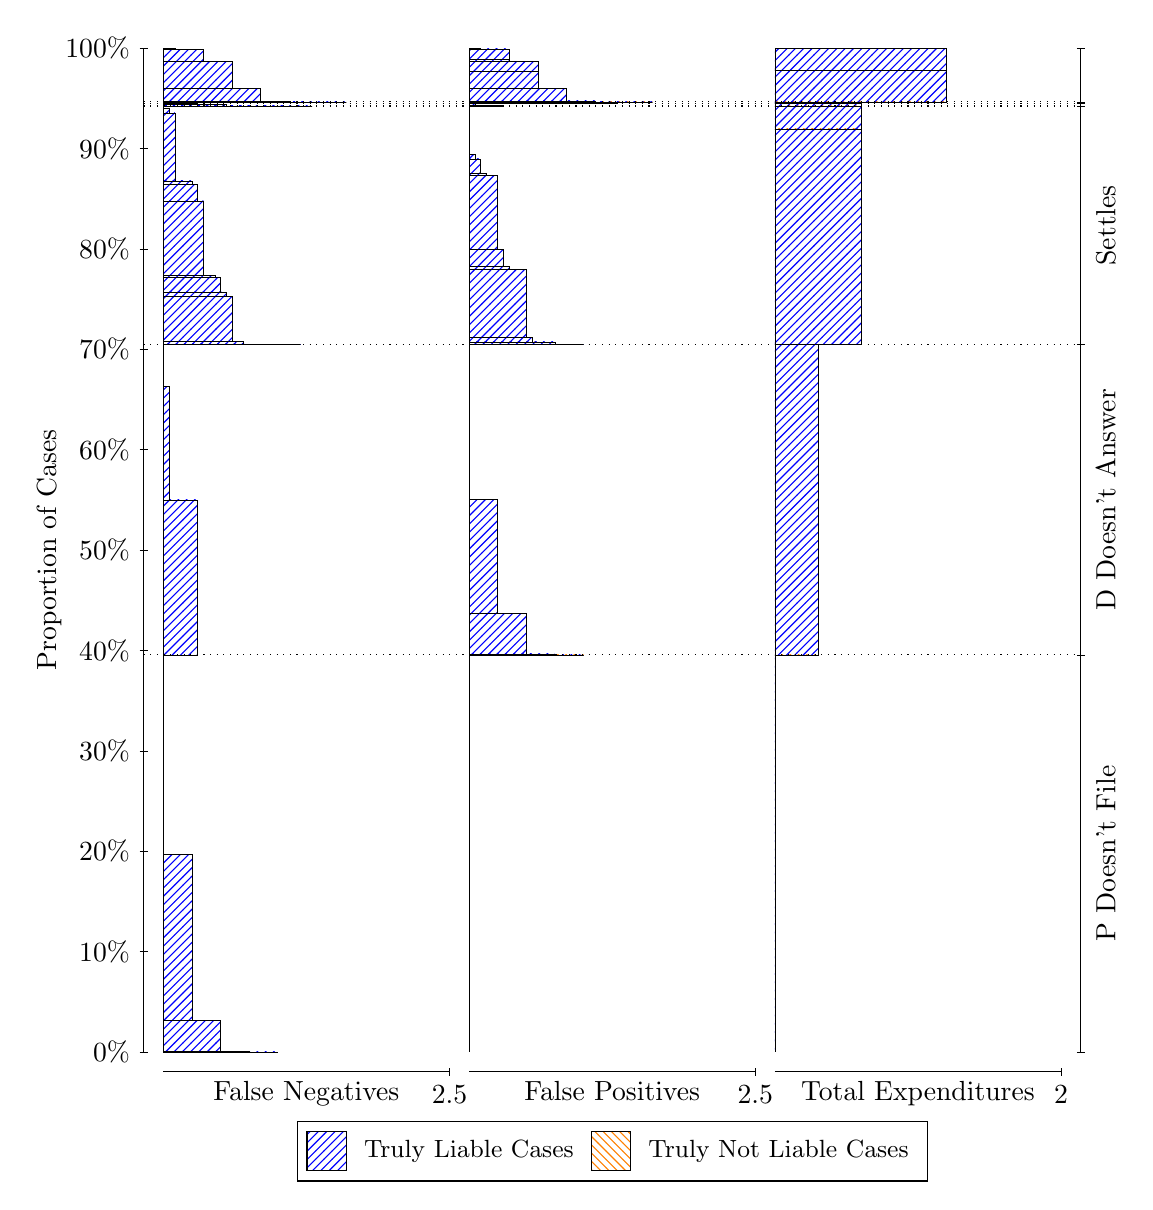
\begin{tikzpicture}
\draw[black, very thin] (1.5,1.75) -- (1.5,14.5);
\node[rotate=90, text=black, anchor=center] at (0.3, 8.125) {Proportion of Cases};
\draw[black, very thin] (1.45,1.75) -- (1.55,1.75);
\node[text=black, anchor=east] at (1.45, 1.75) {0\%};
\draw[black, very thin] (1.45,3.025) -- (1.55,3.025);
\node[text=black, anchor=east] at (1.45, 3.025) {10\%};
\draw[black, very thin] (1.45,4.3) -- (1.55,4.3);
\node[text=black, anchor=east] at (1.45, 4.3) {20\%};
\draw[black, very thin] (1.45,5.575) -- (1.55,5.575);
\node[text=black, anchor=east] at (1.45, 5.575) {30\%};
\draw[black, very thin] (1.45,6.85) -- (1.55,6.85);
\node[text=black, anchor=east] at (1.45, 6.85) {40\%};
\draw[black, very thin] (1.45,8.125) -- (1.55,8.125);
\node[text=black, anchor=east] at (1.45, 8.125) {50\%};
\draw[black, very thin] (1.45,9.4) -- (1.55,9.4);
\node[text=black, anchor=east] at (1.45, 9.4) {60\%};
\draw[black, very thin] (1.45,10.675) -- (1.55,10.675);
\node[text=black, anchor=east] at (1.45, 10.675) {70\%};
\draw[black, very thin] (1.45,11.95) -- (1.55,11.95);
\node[text=black, anchor=east] at (1.45, 11.95) {80\%};
\draw[black, very thin] (1.45,13.225) -- (1.55,13.225);
\node[text=black, anchor=east] at (1.45, 13.225) {90\%};
\draw[black, very thin] (1.45,14.5) -- (1.55,14.5);
\node[text=black, anchor=east] at (1.45, 14.5) {100\%};

\draw[black, very thin] (13.4,1.75) -- (13.4,14.5);
\draw[black, very thin] (13.35,1.75) -- (13.45,1.75);
\node[anchor=west] at (13.35, 1.75) {};
\draw[black, very thin] (13.35,6.7931) -- (13.45,6.7931);
\node[anchor=west] at (13.35, 6.7931) {};
\draw[black, very thin] (13.35,10.733) -- (13.45,10.733);
\node[anchor=west] at (13.35, 10.733) {};
\draw[black, very thin] (13.35,13.764) -- (13.45,13.764);
\node[anchor=west] at (13.35, 13.764) {};
\draw[black, very thin] (13.35,13.794) -- (13.45,13.794);
\node[anchor=west] at (13.35, 13.794) {};
\draw[black, very thin] (13.35,13.816) -- (13.45,13.816);
\node[anchor=west] at (13.35, 13.816) {};
\draw[black, very thin] (13.35,14.5) -- (13.45,14.5);
\node[anchor=west] at (13.35, 14.5) {};

\draw[black, very thin, pattern color=blue, pattern=north east lines] (1.75,1.75) rectangle (3.2033,1.75);
\draw[black, very thin, pattern color=blue, pattern=north east lines] (1.75,1.75) rectangle (2.84,1.7534);
\draw[black, very thin, pattern color=blue, pattern=north east lines] (1.75,1.7534) rectangle (2.4767,2.1495);
\draw[black, very thin, pattern color=blue, pattern=north east lines] (1.75,2.1495) rectangle (2.1133,4.2573);
\draw[black, very thin, pattern color=orange, pattern=north west lines] (1.75,4.2573) rectangle (1.75,4.2573);
\draw[black, very thin, pattern color=blue, pattern=north east lines] (1.75,4.2573) rectangle (1.75,6.7931);
\draw[black, very thin, pattern color=blue, pattern=north east lines] (1.75,6.7931) rectangle (2.186,8.7624);
\draw[black, very thin, pattern color=blue, pattern=north east lines] (1.75,8.7624) rectangle (1.8227,10.206);
\draw[black, very thin, pattern color=orange, pattern=north west lines] (1.75,10.206) rectangle (1.75,10.206);
\draw[black, very thin, pattern color=blue, pattern=north east lines] (1.75,10.206) rectangle (1.75,10.733);
\draw[black, very thin, pattern color=blue, pattern=north east lines] (1.75,10.733) rectangle (3.494,10.733);
\draw[black, very thin, pattern color=blue, pattern=north east lines] (1.75,10.733) rectangle (3.2033,10.733);
\draw[black, very thin, pattern color=blue, pattern=north east lines] (1.75,10.733) rectangle (3.1307,10.734);
\draw[black, very thin, pattern color=blue, pattern=north east lines] (1.75,10.734) rectangle (2.9127,10.736);
\draw[black, very thin, pattern color=blue, pattern=north east lines] (1.75,10.736) rectangle (2.84,10.744);
\draw[black, very thin, pattern color=blue, pattern=north east lines] (1.75,10.744) rectangle (2.7673,10.778);
\draw[black, very thin, pattern color=blue, pattern=north east lines] (1.75,10.778) rectangle (2.622,11.347);
\draw[black, very thin, pattern color=blue, pattern=north east lines] (1.75,11.347) rectangle (2.5493,11.404);
\draw[black, very thin, pattern color=blue, pattern=north east lines] (1.75,11.404) rectangle (2.4767,11.585);
\draw[black, very thin, pattern color=blue, pattern=north east lines] (1.75,11.585) rectangle (2.404,11.611);
\draw[black, very thin, pattern color=blue, pattern=north east lines] (1.75,11.611) rectangle (2.2587,12.559);
\draw[black, very thin, pattern color=blue, pattern=north east lines] (1.75,12.559) rectangle (2.186,12.772);
\draw[black, very thin, pattern color=blue, pattern=north east lines] (1.75,12.772) rectangle (2.1133,12.813);
\draw[black, very thin, pattern color=blue, pattern=north east lines] (1.75,12.813) rectangle (2.0407,12.813);
\draw[black, very thin, pattern color=blue, pattern=north east lines] (1.75,12.813) rectangle (1.8953,13.676);
\draw[black, very thin, pattern color=blue, pattern=north east lines] (1.75,13.676) rectangle (1.8227,13.73);
\draw[black, very thin, pattern color=orange, pattern=north west lines] (1.75,13.73) rectangle (1.75,13.73);
\draw[black, very thin, pattern color=blue, pattern=north east lines] (1.75,13.73) rectangle (1.75,13.764);
\draw[black, very thin, pattern color=blue, pattern=north east lines] (1.75,13.764) rectangle (3.6393,13.764);
\draw[black, very thin, pattern color=blue, pattern=north east lines] (1.75,13.764) rectangle (3.276,13.764);
\draw[black, very thin, pattern color=blue, pattern=north east lines] (1.75,13.764) rectangle (2.9127,13.765);
\draw[black, very thin, pattern color=blue, pattern=north east lines] (1.75,13.765) rectangle (2.5493,13.785);
\draw[black, very thin, pattern color=blue, pattern=north east lines] (1.75,13.785) rectangle (2.186,13.794);
\draw[black, very thin, pattern color=orange, pattern=north west lines] (1.75,13.794) rectangle (1.75,13.794);
\draw[black, very thin, pattern color=blue, pattern=north east lines] (1.75,13.794) rectangle (2.186,13.803);
\draw[black, very thin, pattern color=blue, pattern=north east lines] (1.75,13.803) rectangle (1.8227,13.815);
\draw[black, very thin, pattern color=orange, pattern=north west lines] (1.75,13.815) rectangle (1.75,13.815);
\draw[black, very thin, pattern color=blue, pattern=north east lines] (1.75,13.815) rectangle (1.75,13.816);
\draw[black, very thin, pattern color=blue, pattern=north east lines] (1.75,13.816) rectangle (4.0753,13.816);
\draw[black, very thin, pattern color=blue, pattern=north east lines] (1.75,13.816) rectangle (3.712,13.816);
\draw[black, very thin, pattern color=blue, pattern=north east lines] (1.75,13.816) rectangle (3.3487,13.825);
\draw[black, very thin, pattern color=blue, pattern=north east lines] (1.75,13.825) rectangle (2.9853,13.984);
\draw[black, very thin, pattern color=blue, pattern=north east lines] (1.75,13.984) rectangle (2.622,14.327);
\draw[black, very thin, pattern color=blue, pattern=north east lines] (1.75,14.327) rectangle (2.2587,14.486);
\draw[black, very thin, pattern color=blue, pattern=north east lines] (1.75,14.486) rectangle (1.8953,14.5);
\draw[black, very thin, pattern color=orange, pattern=north west lines] (1.75,14.5) rectangle (1.75,14.5);
\draw[black, very thin, pattern color=blue, pattern=north east lines] (1.75,14.5) rectangle (1.75,14.5);
\draw[black, very thin, pattern color=orange, pattern=north west lines] (5.6333,1.75) rectangle (5.6333,1.75);
\draw[black, very thin, pattern color=blue, pattern=north east lines] (5.6333,1.75) rectangle (5.6333,6.7931);
\draw[black, very thin, pattern color=orange, pattern=north west lines] (5.6333,6.7931) rectangle (7.0867,6.7931);
\draw[black, very thin, pattern color=blue, pattern=north east lines] (5.6333,6.7931) rectangle (7.0867,6.7931);
\draw[black, very thin, pattern color=blue, pattern=north east lines] (5.6333,6.7931) rectangle (6.7233,6.807);
\draw[black, very thin, pattern color=blue, pattern=north east lines] (5.6333,6.807) rectangle (6.36,7.3205);
\draw[black, very thin, pattern color=blue, pattern=north east lines] (5.6333,7.3205) rectangle (5.9967,8.764);
\draw[black, very thin, pattern color=blue, pattern=north east lines] (5.6333,8.764) rectangle (5.6333,10.733);
\draw[black, very thin, pattern color=orange, pattern=north west lines] (5.6333,10.733) rectangle (7.0867,10.733);
\draw[black, very thin, pattern color=blue, pattern=north east lines] (5.6333,10.733) rectangle (7.0867,10.733);
\draw[black, very thin, pattern color=orange, pattern=north west lines] (5.6333,10.733) rectangle (6.796,10.733);
\draw[black, very thin, pattern color=blue, pattern=north east lines] (5.6333,10.733) rectangle (6.796,10.735);
\draw[black, very thin, pattern color=blue, pattern=north east lines] (5.6333,10.735) rectangle (6.7233,10.767);
\draw[black, very thin, pattern color=orange, pattern=north west lines] (5.6333,10.767) rectangle (6.5053,10.767);
\draw[black, very thin, pattern color=blue, pattern=north east lines] (5.6333,10.767) rectangle (6.5053,10.767);
\draw[black, very thin, pattern color=blue, pattern=north east lines] (5.6333,10.767) rectangle (6.4327,10.821);
\draw[black, very thin, pattern color=blue, pattern=north east lines] (5.6333,10.821) rectangle (6.36,11.684);
\draw[black, very thin, pattern color=orange, pattern=north west lines] (5.6333,11.684) rectangle (6.2147,11.684);
\draw[black, very thin, pattern color=blue, pattern=north east lines] (5.6333,11.684) rectangle (6.2147,11.684);
\draw[black, very thin, pattern color=blue, pattern=north east lines] (5.6333,11.684) rectangle (6.142,11.724);
\draw[black, very thin, pattern color=blue, pattern=north east lines] (5.6333,11.724) rectangle (6.0693,11.938);
\draw[black, very thin, pattern color=blue, pattern=north east lines] (5.6333,11.938) rectangle (5.9967,12.886);
\draw[black, very thin, pattern color=blue, pattern=north east lines] (5.6333,12.886) rectangle (5.8513,12.912);
\draw[black, very thin, pattern color=blue, pattern=north east lines] (5.6333,12.912) rectangle (5.7787,13.093);
\draw[black, very thin, pattern color=blue, pattern=north east lines] (5.6333,13.093) rectangle (5.706,13.15);
\draw[black, very thin, pattern color=blue, pattern=north east lines] (5.6333,13.15) rectangle (5.6333,13.764);
\draw[black, very thin, pattern color=orange, pattern=north west lines] (5.6333,13.764) rectangle (6.0693,13.764);
\draw[black, very thin, pattern color=blue, pattern=north east lines] (5.6333,13.764) rectangle (6.0693,13.773);
\draw[black, very thin, pattern color=blue, pattern=north east lines] (5.6333,13.773) rectangle (5.706,13.792);
\draw[black, very thin, pattern color=blue, pattern=north east lines] (5.6333,13.792) rectangle (5.6333,13.794);
\draw[black, very thin, pattern color=orange, pattern=north west lines] (5.6333,13.794) rectangle (7.5227,13.794);
\draw[black, very thin, pattern color=blue, pattern=north east lines] (5.6333,13.794) rectangle (7.5227,13.794);
\draw[black, very thin, pattern color=blue, pattern=north east lines] (5.6333,13.794) rectangle (7.1593,13.794);
\draw[black, very thin, pattern color=blue, pattern=north east lines] (5.6333,13.794) rectangle (6.796,13.795);
\draw[black, very thin, pattern color=blue, pattern=north east lines] (5.6333,13.795) rectangle (6.4327,13.807);
\draw[black, very thin, pattern color=blue, pattern=north east lines] (5.6333,13.807) rectangle (6.0693,13.816);
\draw[black, very thin, pattern color=orange, pattern=north west lines] (5.6333,13.816) rectangle (7.9587,13.816);
\draw[black, very thin, pattern color=blue, pattern=north east lines] (5.6333,13.816) rectangle (7.9587,13.816);
\draw[black, very thin, pattern color=orange, pattern=north west lines] (5.6333,13.816) rectangle (7.5953,13.816);
\draw[black, very thin, pattern color=blue, pattern=north east lines] (5.6333,13.816) rectangle (7.5953,13.816);
\draw[black, very thin, pattern color=orange, pattern=north west lines] (5.6333,13.816) rectangle (7.232,13.816);
\draw[black, very thin, pattern color=blue, pattern=north east lines] (5.6333,13.816) rectangle (7.232,13.83);
\draw[black, very thin, pattern color=blue, pattern=north east lines] (5.6333,13.83) rectangle (6.8687,13.988);
\draw[black, very thin, pattern color=orange, pattern=north west lines] (5.6333,13.988) rectangle (6.8687,13.988);
\draw[black, very thin, pattern color=blue, pattern=north east lines] (5.6333,13.988) rectangle (6.8687,13.989);
\draw[black, very thin, pattern color=blue, pattern=north east lines] (5.6333,13.989) rectangle (6.5053,14.2);
\draw[black, very thin, pattern color=orange, pattern=north west lines] (5.6333,14.2) rectangle (6.5053,14.2);
\draw[black, very thin, pattern color=blue, pattern=north east lines] (5.6333,14.2) rectangle (6.5053,14.332);
\draw[black, very thin, pattern color=blue, pattern=north east lines] (5.6333,14.332) rectangle (6.142,14.351);
\draw[black, very thin, pattern color=blue, pattern=north east lines] (5.6333,14.351) rectangle (6.142,14.49);
\draw[black, very thin, pattern color=blue, pattern=north east lines] (5.6333,14.49) rectangle (5.7787,14.49);
\draw[black, very thin, pattern color=blue, pattern=north east lines] (5.6333,14.49) rectangle (5.7787,14.5);
\draw[black, very thin, pattern color=blue, pattern=north east lines] (5.6333,14.5) rectangle (5.6333,14.5);
\draw[black, very thin, pattern color=orange, pattern=north west lines] (9.5167,1.75) rectangle (9.5167,1.75);
\draw[black, very thin, pattern color=blue, pattern=north east lines] (9.5167,1.75) rectangle (9.5167,6.7931);
\draw[black, very thin, pattern color=orange, pattern=north west lines] (9.5167,6.7931) rectangle (10.062,6.7931);
\draw[black, very thin, pattern color=blue, pattern=north east lines] (9.5167,6.7931) rectangle (10.062,10.733);
\draw[black, very thin, pattern color=orange, pattern=north west lines] (9.5167,10.733) rectangle (10.607,10.733);
\draw[black, very thin, pattern color=blue, pattern=north east lines] (9.5167,10.733) rectangle (10.607,13.473);
\draw[black, very thin, pattern color=orange, pattern=north west lines] (9.5167,13.473) rectangle (10.607,13.473);
\draw[black, very thin, pattern color=blue, pattern=north east lines] (9.5167,13.473) rectangle (10.607,13.764);
\draw[black, very thin, pattern color=orange, pattern=north west lines] (9.5167,13.764) rectangle (10.607,13.764);
\draw[black, very thin, pattern color=blue, pattern=north east lines] (9.5167,13.764) rectangle (10.607,13.794);
\draw[black, very thin, pattern color=orange, pattern=north west lines] (9.5167,13.794) rectangle (10.607,13.794);
\draw[black, very thin, pattern color=blue, pattern=north east lines] (9.5167,13.794) rectangle (10.607,13.816);
\draw[black, very thin, pattern color=orange, pattern=north west lines] (9.5167,13.816) rectangle (11.697,13.816);
\draw[black, very thin, pattern color=blue, pattern=north east lines] (9.5167,13.816) rectangle (11.697,14.217);
\draw[black, very thin, pattern color=orange, pattern=north west lines] (9.5167,14.217) rectangle (11.697,14.217);
\draw[black, very thin, pattern color=blue, pattern=north east lines] (9.5167,14.217) rectangle (11.697,14.5);
\draw[black, dotted] (1.5,6.7931) -- (13.4,6.7931);
\draw[black, dotted] (1.5,10.733) -- (13.4,10.733);
\draw[black, dotted] (1.5,13.764) -- (13.4,13.764);
\draw[black, dotted] (1.5,13.794) -- (13.4,13.794);
\draw[black, dotted] (1.5,13.816) -- (13.4,13.816);
\draw[black, very thin] (1.75,1.5) -- (5.3833,1.5);
\node[text=black, anchor=north] at (3.5667, 1.5) {False Negatives};
\draw[black, very thin] (5.3833,1.45) -- (5.3833,1.55);
\node[text=black, anchor=north] at (5.3833, 1.45) {2.5};

\draw[black, very thin] (5.6333,1.5) -- (9.2667,1.5);
\node[text=black, anchor=north] at (7.45, 1.5) {False Positives};
\draw[black, very thin] (9.2667,1.45) -- (9.2667,1.55);
\node[text=black, anchor=north] at (9.2667, 1.45) {2.5};

\draw[black, very thin] (9.5167,1.5) -- (13.15,1.5);
\node[text=black, anchor=north] at (11.333, 1.5) {Total Expenditures};
\draw[black, very thin] (13.15,1.45) -- (13.15,1.55);
\node[text=black, anchor=north] at (13.15, 1.45) {2};

\node[text=black, centered, rotate=90] at (13.72, 4.2716) {P Doesn't File};
\node[text=black, centered, rotate=90] at (13.72, 8.7632) {D Doesn't Answer};
\node[text=black, centered, rotate=90] at (13.72, 12.248) {Settles};




\draw (7.449999999999999,1.5) node[draw=none] (baseCoordinate) {};
\begin{scope}[align=center]
        \matrix[scale=0.5, draw=black, below=0.5cm of baseCoordinate, nodes={draw}, column sep=0.1cm]{
            \node[rectangle, draw, minimum width=0.5cm, minimum height=0.5cm, pattern color=blue, pattern=north east lines] {}; &
            \node[draw=none, font=\small, text=black] (B) {Truly Liable Cases}; &
            \node[rectangle, draw, minimum width=0.5cm, minimum height=0.5cm, pattern color=orange, pattern=north west lines] {}; &
            \node[draw=none, font=\small, text=black] (B) {Truly Not Liable Cases}; \\
            };
\end{scope}

\end{tikzpicture}
\end{document}